\documentclass[12pt]{article}
%Gummi|065|=)
\usepackage{amsmath, amsfonts, amssymb}
\usepackage[margin=0.5in]{geometry}
\usepackage{xcolor}
%\usepackage{graphicx}
%\usepackage{graphicx}
\newcommand{\off}[1]{}
\DeclareMathSizes{20}{30}{21}{18}

\newcommand{\myhrule}{}

\newcommand{\dash}{
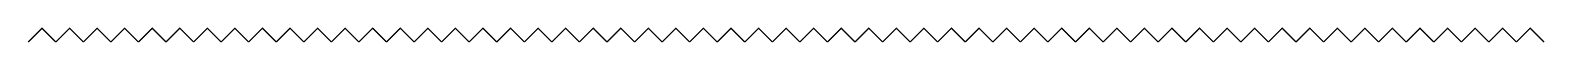
\begin{tikzpicture}[scale=0.35]
\foreach \x in {1,...,55}{
	\draw (\x,-0.25)--(\x+0.5,0.25)--(\x+1,-0.25);
}
\end{tikzpicture}
}

\usepackage{tikz}

\title{\textbf{ Examples:  Quadratic Reciprocity}}
\author{John D Mangual}
\date{}
\begin{document}

\fontfamily{qag}\selectfont \fontsize{25}{30}\selectfont

\maketitle

\noindent Here is a theorem from the modern number theory literature (about 10 years old):\footnote{Akshay Venkatesh -- Sparese Equdistribution Problems, Period Bounds and Subconvexity -- \textit{Annals of Mathematics} (2005)}

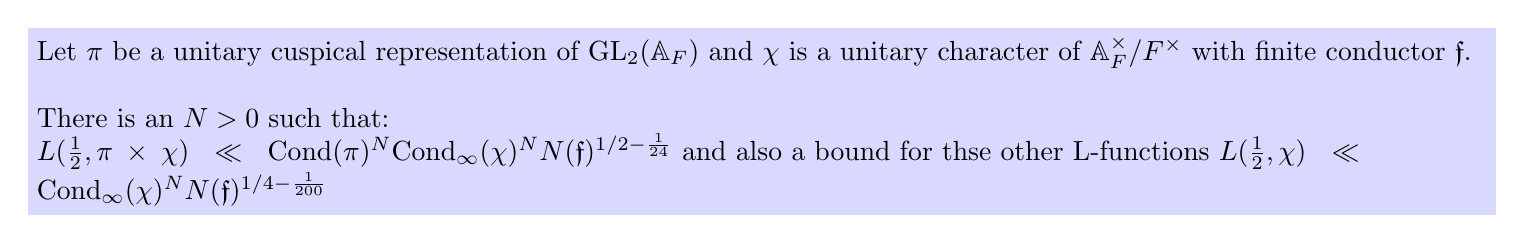
\begin{tikzpicture}
\node[text width=7.25in, fill=blue!15!white] at (0,0){
Let $\pi$ be a unitary cuspical representation of $\mathrm{GL}_2(\mathbb{A}_F)$ and $\chi$ is a unitary character of $\mathbb{A}_F^\times / F^\times$ with finite conductor $\mathfrak{f}$. \\ \vspace{12pt} There is an $N > 0$ such that: \\
$L(\frac{1}{2}, \pi \times \chi) \ll \mathrm{Cond}(\pi)^N \mathrm{Cond}_\infty (\chi)^N N(\mathfrak{f})^{1/2 - \frac{1}{24}} $ 
and also a bound for thse other L-functions
$L(\frac{1}{2}, \chi) \ll  \mathrm{Cond}_\infty (\chi)^N N(\mathfrak{f})^{1/4 - \frac{1}{200}} $};
\end{tikzpicture}
This is unfortunately written at such a level of abstraction that we have no idea what is going on.   \\ \\
I barely know what a modular form or an L-function is (though I am seeing them constantly)  \newpage

\noindent Then the author says if we set $F = \mathbb{Q}$ this is a \textit{subconvexity} result due to Burgess.  \\ \\
I know what ``convex" means - a circle is convex.  A square is convex.  I don't know what \textbf{subconvex} means. \\ \\
Burgess proved $L(\frac{1}{2}, \chi) \ll k^{\frac{7}{32}+\epsilon} $ and the ``principal difficulty" [Burgess' words] is to show an estimate like this:
$$ \sum_{x=1}^k \bigg| \sum_{y=1}^h \chi(x+y) \bigg|^{2r} $$
here $\chi$ is a Dirichlet charcter (such the Legendre symbol $(\frac{\cdot}{p})$. \\ \\
There is nothing convex about this. And in a way it doesn't matter since we can write down the formula:
$$ L( \frac{1}{2}, \chi) = \sum_{n = 1}^\infty \frac{\chi(n)}{\sqrt{n}} $$
This is divergent if $\chi \equiv 1$ -- the \textbf{trivial character} but what about other sequences of $\pm 1$ ?


\newpage

\noindent  \textbf{\#1} - For every number there can be a Dirichlet character.  Mod 3 we can set $\chi(2)=-1$ and then
$$ L(\tfrac{1}{2}, \chi_3) = 
0+
\frac{1}{\sqrt{1}} - 
 \frac{1}{\sqrt{2}} +
 0 + 
\frac{1}{\sqrt{4}} - 
 \frac{1}{\sqrt{5}} +
 0 + \dots 
$$
and this symbol ``$\ll$" is somewhat startling since are are not looking at any single Dirichlet characters, but \textit{all} Dirichlet characters as $k \to \infty$.  \\ \\
Those numbers $L(\frac{1}{2}, \chi) \ll k^\frac{7}{24}$ (or whatever crazy exponent you will put). \\ \\
\noindent  \textbf{\#2} - Subconvexity bounds - admittedly not very convex - originate from 
\begin{itemize}
\item the \textbf{Phragmen-Lindel\"{o}f} theorem and
\item the \textbf{Hadamard three circles} theorem 
\item The \textbf{Maximum Modulus} theorem
\end{itemize}
as I found out flipping between various textbooks\footnote{If you know which book to look at, it is easy to get started.  These are the resoures I found.  Actually quite old. \\ Titchmarsh \textbf{Theory of Functions} (endlessly useful - I thought I knew it all already)  \\ Iwaniec + Kowalski \textbf{Analytic Number Theory} The maximum modulus principle talks about \textbf{bounded holomorphic functions} if $|f(z) \leq M$ on $C$ either:\begin{itemize}
\item $|f(z)|< M$ at all interior points in $D$
\item $f(z)\equiv M$ is a constant.
\end{itemize}  }

\newpage

\noindent \textbf{\#3} - This might be the wrong idea but I would like to study the equation 
$$ x^2 + y^2 + z^2 = d $$
The number of three squares points is related to the 
$$ \# \big\{ (x,y,z): x^2 + y^2 + z^2 = n \big\}
=  \frac{24}{\pi} \sqrt{n} L (1, \chi_{n \text{ or }4n})$$
These numbers should be very roughly evenly distributed on the sphere, but there are still many patterns which persist for large values $d \gg 1$. \\ \\
And $L(1, \chi)$ is a slightly different series.  
$$ \sum \frac{\chi(n)}{n} < n^{\frac{1}{2} + \epsilon} $$
and if $\chi \equiv 1$ this series is the \textbf{Harmonic series} which is divergent.  \\ \\
Yet, I have to keep my L-functions straight.  $L(\frac{1}{2}, \chi)$ and $L(1, \chi)$.  When is one appropriate and when is the other?

\newpage

\fontfamily{qag}\selectfont \fontsize{12}{10}\selectfont


\begin{thebibliography}{}

\item Jared Weinstein. \textbf{Reciprocity laws and Galois representations: recent breakthroughs} Bull. Amer. Math. Soc. 53 (2016), 1-39 

\item David A Cox. \textbf{Primes of the Form $x^2+ny^2$: Fermat, Class Field Theory, and Complex Multiplication} Wiley, 2013.

\item \textbf{A prime ideal $\mathfrak{p}$ decomposes in $\mathbb{Q}(\zeta_{24})/\mathbb{Q}(\sqrt{-6})$ iff it is generated by $\alpha\in1+2\Bbb{Z}[\sqrt{-6}]$} \\ \texttt{http://mathoverflow.net/q/234570/1358}

\item Roy L. Adler \textbf{Symbolic dynamics and Markov partitions}  Bull. Amer. Math. Soc. 35 (1998), 1-56  \\ \texttt{http://www.ams.org/journals/bull/1998-35-01/S0273-0979-98-00737-X/}


\end{thebibliography}



\end{document}